\documentclass[twoside]{book}

% Packages required by doxygen
\usepackage{fixltx2e}
\usepackage{calc}
\usepackage{doxygen}
\usepackage[export]{adjustbox} % also loads graphicx
\usepackage{graphicx}
\usepackage[utf8]{inputenc}
\usepackage{makeidx}
\usepackage{multicol}
\usepackage{multirow}
\PassOptionsToPackage{warn}{textcomp}
\usepackage{textcomp}
\usepackage[nointegrals]{wasysym}
\usepackage[table]{xcolor}

% Font selection
\usepackage[T1]{fontenc}
\usepackage[scaled=.90]{helvet}
\usepackage{courier}
\usepackage{amssymb}
\usepackage{sectsty}
\renewcommand{\familydefault}{\sfdefault}
\allsectionsfont{%
  \fontseries{bc}\selectfont%
  \color{darkgray}%
}
\renewcommand{\DoxyLabelFont}{%
  \fontseries{bc}\selectfont%
  \color{darkgray}%
}
\newcommand{\+}{\discretionary{\mbox{\scriptsize$\hookleftarrow$}}{}{}}

% Page & text layout
\usepackage{geometry}
\geometry{%
  a4paper,%
  top=2.5cm,%
  bottom=2.5cm,%
  left=2.5cm,%
  right=2.5cm%
}
\tolerance=750
\hfuzz=15pt
\hbadness=750
\setlength{\emergencystretch}{15pt}
\setlength{\parindent}{0cm}
\setlength{\parskip}{0.2cm}
\makeatletter
\renewcommand{\paragraph}{%
  \@startsection{paragraph}{4}{0ex}{-1.0ex}{1.0ex}{%
    \normalfont\normalsize\bfseries\SS@parafont%
  }%
}
\renewcommand{\subparagraph}{%
  \@startsection{subparagraph}{5}{0ex}{-1.0ex}{1.0ex}{%
    \normalfont\normalsize\bfseries\SS@subparafont%
  }%
}
\makeatother

% Headers & footers
\usepackage{fancyhdr}
\pagestyle{fancyplain}
\fancyhead[LE]{\fancyplain{}{\bfseries\thepage}}
\fancyhead[CE]{\fancyplain{}{}}
\fancyhead[RE]{\fancyplain{}{\bfseries\leftmark}}
\fancyhead[LO]{\fancyplain{}{\bfseries\rightmark}}
\fancyhead[CO]{\fancyplain{}{}}
\fancyhead[RO]{\fancyplain{}{\bfseries\thepage}}
\fancyfoot[LE]{\fancyplain{}{}}
\fancyfoot[CE]{\fancyplain{}{}}
\fancyfoot[RE]{\fancyplain{}{\bfseries\scriptsize Generated on Mon Jun 22 2015 19\+:13\+:30 for Investment\+Analysis\+Diploma by Doxygen }}
\fancyfoot[LO]{\fancyplain{}{\bfseries\scriptsize Generated on Mon Jun 22 2015 19\+:13\+:30 for Investment\+Analysis\+Diploma by Doxygen }}
\fancyfoot[CO]{\fancyplain{}{}}
\fancyfoot[RO]{\fancyplain{}{}}
\renewcommand{\footrulewidth}{0.4pt}
\renewcommand{\chaptermark}[1]{%
  \markboth{#1}{}%
}
\renewcommand{\sectionmark}[1]{%
  \markright{\thesection\ #1}%
}

% Indices & bibliography
\usepackage{natbib}
\usepackage[titles]{tocloft}
\setcounter{tocdepth}{3}
\setcounter{secnumdepth}{5}
\makeindex

% Hyperlinks (required, but should be loaded last)
\usepackage{ifpdf}
\ifpdf
  \usepackage[pdftex,pagebackref=true]{hyperref}
\else
  \usepackage[ps2pdf,pagebackref=true]{hyperref}
\fi
\hypersetup{%
  colorlinks=true,%
  linkcolor=blue,%
  citecolor=blue,%
  unicode%
}

% Custom commands
\newcommand{\clearemptydoublepage}{%
  \newpage{\pagestyle{empty}\cleardoublepage}%
}


%===== C O N T E N T S =====

\begin{document}

% Titlepage & ToC
\hypersetup{pageanchor=false,
             bookmarks=true,
             bookmarksnumbered=true,
             pdfencoding=unicode
            }
\pagenumbering{roman}
\begin{titlepage}
\vspace*{7cm}
\begin{center}%
{\Large Investment\+Analysis\+Diploma }\\
\vspace*{1cm}
{\large Generated by Doxygen 1.8.9.1}\\
\vspace*{0.5cm}
{\small Mon Jun 22 2015 19:13:30}\\
\end{center}
\end{titlepage}
\clearemptydoublepage
\tableofcontents
\clearemptydoublepage
\pagenumbering{arabic}
\hypersetup{pageanchor=true}

%--- Begin generated contents ---
\chapter{Hierarchical Index}
\section{Class Hierarchy}
This inheritance list is sorted roughly, but not completely, alphabetically\+:\begin{DoxyCompactList}
\item \contentsline{section}{Cash\+Flow}{\pageref{class_cash_flow}}{}
\item \contentsline{section}{Credit}{\pageref{class_credit}}{}
\item \contentsline{section}{Economical\+Situation}{\pageref{class_economical_situation}}{}
\item \contentsline{section}{Investment\+Portfolio}{\pageref{class_investment_portfolio}}{}
\item \contentsline{section}{Investment\+Project}{\pageref{class_investment_project}}{}
\item \contentsline{section}{Investor}{\pageref{class_investor}}{}
\item Q\+Main\+Window\begin{DoxyCompactList}
\item \contentsline{section}{Input\+Module}{\pageref{class_input_module}}{}
\end{DoxyCompactList}
\item \contentsline{section}{qt\+\_\+meta\+\_\+stringdata\+\_\+\+Input\+Module\+\_\+t}{\pageref{structqt__meta__stringdata___input_module__t}}{}
\item \contentsline{section}{Stock}{\pageref{class_stock}}{}
\item \contentsline{section}{Ui\+\_\+\+Input\+Module}{\pageref{class_ui___input_module}}{}
\begin{DoxyCompactList}
\item \contentsline{section}{Ui\+:\+:Input\+Module}{\pageref{class_ui_1_1_input_module}}{}
\end{DoxyCompactList}
\end{DoxyCompactList}

\chapter{Class Index}
\section{Class List}
Here are the classes, structs, unions and interfaces with brief descriptions\+:\begin{DoxyCompactList}
\item\contentsline{section}{\hyperlink{class_cash_flow}{Cash\+Flow} }{\pageref{class_cash_flow}}{}
\item\contentsline{section}{\hyperlink{class_credit}{Credit} }{\pageref{class_credit}}{}
\item\contentsline{section}{\hyperlink{class_economical_situation}{Economical\+Situation} }{\pageref{class_economical_situation}}{}
\item\contentsline{section}{\hyperlink{class_ui_1_1_input_module}{Ui\+::\+Input\+Module} }{\pageref{class_ui_1_1_input_module}}{}
\item\contentsline{section}{\hyperlink{class_input_module}{Input\+Module} }{\pageref{class_input_module}}{}
\item\contentsline{section}{\hyperlink{class_investment_portfolio}{Investment\+Portfolio} }{\pageref{class_investment_portfolio}}{}
\item\contentsline{section}{\hyperlink{class_investment_project}{Investment\+Project} }{\pageref{class_investment_project}}{}
\item\contentsline{section}{\hyperlink{class_investor}{Investor} }{\pageref{class_investor}}{}
\item\contentsline{section}{\hyperlink{structqt__meta__stringdata___input_module__t}{qt\+\_\+meta\+\_\+stringdata\+\_\+\+Input\+Module\+\_\+t} }{\pageref{structqt__meta__stringdata___input_module__t}}{}
\item\contentsline{section}{\hyperlink{class_stock}{Stock} }{\pageref{class_stock}}{}
\item\contentsline{section}{\hyperlink{class_ui___input_module}{Ui\+\_\+\+Input\+Module} }{\pageref{class_ui___input_module}}{}
\end{DoxyCompactList}

\chapter{Class Documentation}
\hypertarget{class_cash_flow}{}\section{Cash\+Flow Class Reference}
\label{class_cash_flow}\index{Cash\+Flow@{Cash\+Flow}}
\subsection*{Public Member Functions}
\begin{DoxyCompactItemize}
\item 
\hypertarget{class_cash_flow_a763513884417f8495925752b02a8c77a}{}double {\bfseries profit} () const \label{class_cash_flow_a763513884417f8495925752b02a8c77a}

\item 
\hypertarget{class_cash_flow_adf551f6d27865350608dcef7e2d8ccca}{}void {\bfseries set\+Profit} (double profit)\label{class_cash_flow_adf551f6d27865350608dcef7e2d8ccca}

\item 
\hypertarget{class_cash_flow_a53f108f0ccbffc449eb6a457cb57b637}{}double {\bfseries expense} () const \label{class_cash_flow_a53f108f0ccbffc449eb6a457cb57b637}

\item 
\hypertarget{class_cash_flow_aae85ccdf2e3663c2aaa581df8b1c4f9c}{}void {\bfseries set\+Expense} (double expense)\label{class_cash_flow_aae85ccdf2e3663c2aaa581df8b1c4f9c}

\item 
\hypertarget{class_cash_flow_a42eb3f91615e8676b90b50d8c75c13de}{}int {\bfseries year} () const \label{class_cash_flow_a42eb3f91615e8676b90b50d8c75c13de}

\item 
\hypertarget{class_cash_flow_af21bc111a3a89624a9989723b291da5b}{}void {\bfseries set\+Year} (int year)\label{class_cash_flow_af21bc111a3a89624a9989723b291da5b}

\end{DoxyCompactItemize}


The documentation for this class was generated from the following files\+:\begin{DoxyCompactItemize}
\item 
C\+:/\+Users/\+Anton/\+Documents/\+Qt\+Projects/\+Investment\+Analysis\+Diploma/cashflow.\+h\item 
C\+:/\+Users/\+Anton/\+Documents/\+Qt\+Projects/\+Investment\+Analysis\+Diploma/cashflow.\+cpp\end{DoxyCompactItemize}

\hypertarget{class_credit}{}\section{Credit Class Reference}
\label{class_credit}\index{Credit@{Credit}}
\subsection*{Public Member Functions}
\begin{DoxyCompactItemize}
\item 
\hypertarget{class_credit_a0ba28d10c484b0a6d42a3b44119dd209}{}Q\+String {\bfseries bank\+Name} () const \label{class_credit_a0ba28d10c484b0a6d42a3b44119dd209}

\item 
\hypertarget{class_credit_a32b7b7e7b66b9c7c870ae4034994cb1e}{}void {\bfseries set\+Bank\+Name} (const Q\+String \&bank\+Name)\label{class_credit_a32b7b7e7b66b9c7c870ae4034994cb1e}

\item 
\hypertarget{class_credit_ad4fb475785f21596d5fdbb7ffa12b8d3}{}double {\bfseries credit\+Rate} () const \label{class_credit_ad4fb475785f21596d5fdbb7ffa12b8d3}

\item 
\hypertarget{class_credit_a2a08e48a7e87086b0cd1719fff123cfc}{}void {\bfseries set\+Credit\+Rate} (double credit\+Rate)\label{class_credit_a2a08e48a7e87086b0cd1719fff123cfc}

\item 
\hypertarget{class_credit_a37fe976e4d33c40db5a2be2e5ce4ea6d}{}double {\bfseries credit\+Value} () const \label{class_credit_a37fe976e4d33c40db5a2be2e5ce4ea6d}

\item 
\hypertarget{class_credit_acf22df48a1619f8a6210d473921ae801}{}void {\bfseries set\+Credit\+Value} (double credit\+Value)\label{class_credit_acf22df48a1619f8a6210d473921ae801}

\item 
\hypertarget{class_credit_ac21c56a88a57483392c1c96d466f03a5}{}int {\bfseries repayment\+Period} () const \label{class_credit_ac21c56a88a57483392c1c96d466f03a5}

\item 
\hypertarget{class_credit_a2496520ec0cfc37a832bd4861b6168cc}{}void {\bfseries set\+Repayment\+Period} (int repayment\+Period)\label{class_credit_a2496520ec0cfc37a832bd4861b6168cc}

\end{DoxyCompactItemize}


The documentation for this class was generated from the following files\+:\begin{DoxyCompactItemize}
\item 
C\+:/\+Users/\+Anton/\+Documents/\+Qt\+Projects/\+Investment\+Analysis\+Diploma/credit.\+h\item 
C\+:/\+Users/\+Anton/\+Documents/\+Qt\+Projects/\+Investment\+Analysis\+Diploma/credit.\+cpp\end{DoxyCompactItemize}

\hypertarget{class_economical_situation}{}\section{Economical\+Situation Class Reference}
\label{class_economical_situation}\index{Economical\+Situation@{Economical\+Situation}}
\subsection*{Public Member Functions}
\begin{DoxyCompactItemize}
\item 
\hypertarget{class_economical_situation_acfb33013935115d19f5ac6e90da45c5f}{}double {\bfseries inflation\+Rate} () const \label{class_economical_situation_acfb33013935115d19f5ac6e90da45c5f}

\item 
\hypertarget{class_economical_situation_a266ce3329863b711505ea165f64eee91}{}void {\bfseries set\+Inflation\+Rate} (double inflation\+Rate)\label{class_economical_situation_a266ce3329863b711505ea165f64eee91}

\item 
\hypertarget{class_economical_situation_a7b5a02539cf70475c7423e1f685650e0}{}double {\bfseries basic\+Rate} () const \label{class_economical_situation_a7b5a02539cf70475c7423e1f685650e0}

\item 
\hypertarget{class_economical_situation_a9b20a41fc26c8e730331b645bb842528}{}void {\bfseries set\+Basic\+Rate} (double basic\+Rate)\label{class_economical_situation_a9b20a41fc26c8e730331b645bb842528}

\item 
\hypertarget{class_economical_situation_a7e4860654676d934a6db253d7e37fcd4}{}double {\bfseries discount\+Rate} () const \label{class_economical_situation_a7e4860654676d934a6db253d7e37fcd4}

\item 
\hypertarget{class_economical_situation_a053d360a6ba097bd1b438b5d21bd7bdb}{}void {\bfseries set\+Discount\+Rate} (double discount\+Rate)\label{class_economical_situation_a053d360a6ba097bd1b438b5d21bd7bdb}

\item 
\hypertarget{class_economical_situation_abdcd91b38707d72a13550e450fe48147}{}double {\bfseries profit\+Tax\+Rate} () const \label{class_economical_situation_abdcd91b38707d72a13550e450fe48147}

\item 
\hypertarget{class_economical_situation_a03998405c058bbb8a8e078ef0d101f46}{}void {\bfseries set\+Profit\+Tax\+Rate} (double profit\+Tax\+Rate)\label{class_economical_situation_a03998405c058bbb8a8e078ef0d101f46}

\end{DoxyCompactItemize}


The documentation for this class was generated from the following files\+:\begin{DoxyCompactItemize}
\item 
C\+:/\+Users/\+Anton/\+Documents/\+Qt\+Projects/\+Investment\+Analysis\+Diploma/economicalsituation.\+h\item 
C\+:/\+Users/\+Anton/\+Documents/\+Qt\+Projects/\+Investment\+Analysis\+Diploma/economicalsituation.\+cpp\end{DoxyCompactItemize}

\hypertarget{class_ui_1_1_input_module}{}\section{Ui\+:\+:Input\+Module Class Reference}
\label{class_ui_1_1_input_module}\index{Ui\+::\+Input\+Module@{Ui\+::\+Input\+Module}}
Inheritance diagram for Ui\+:\+:Input\+Module\+:\begin{figure}[H]
\begin{center}
\leavevmode
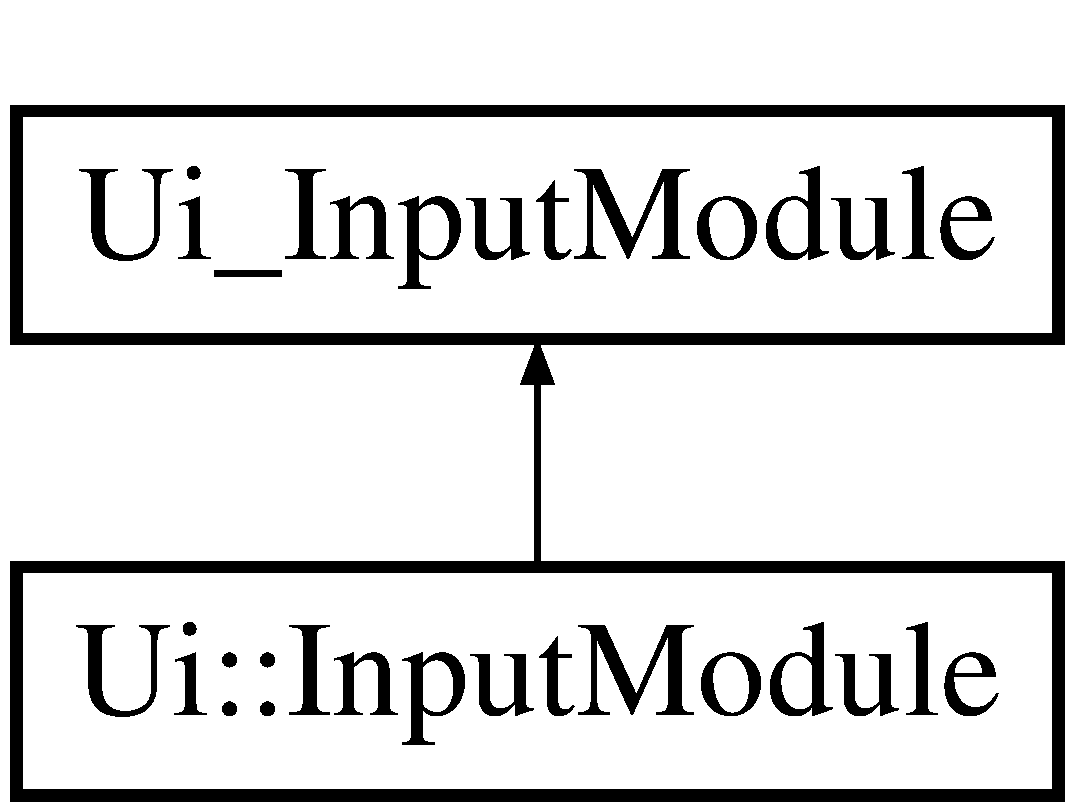
\includegraphics[height=2.000000cm]{class_ui_1_1_input_module}
\end{center}
\end{figure}
\subsection*{Additional Inherited Members}


The documentation for this class was generated from the following file\+:\begin{DoxyCompactItemize}
\item 
C\+:/\+Users/\+Anton/\+Documents/\+Qt\+Projects/\+Investment\+Analysis\+Diploma/ui\+\_\+inputmodule.\+h\end{DoxyCompactItemize}

\hypertarget{class_input_module}{}\section{Input\+Module Class Reference}
\label{class_input_module}\index{Input\+Module@{Input\+Module}}
Inheritance diagram for Input\+Module\+:\begin{figure}[H]
\begin{center}
\leavevmode
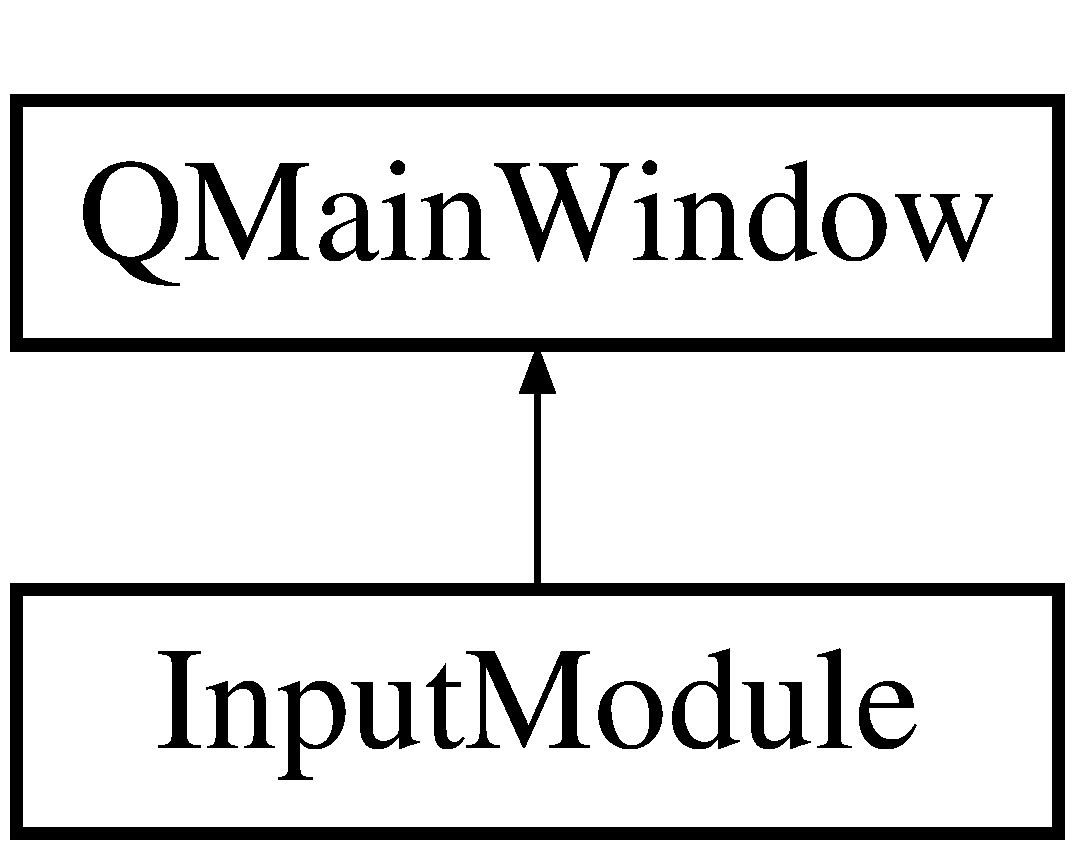
\includegraphics[height=2.000000cm]{class_input_module}
\end{center}
\end{figure}
\subsection*{Public Slots}
\begin{DoxyCompactItemize}
\item 
\hypertarget{class_input_module_a98a75cba7c65889bc27d5f052693a975}{}void {\bfseries add\+Column} (int column)\label{class_input_module_a98a75cba7c65889bc27d5f052693a975}

\item 
\hypertarget{class_input_module_aa344a18931623103e86a47499b0c9577}{}void {\bfseries delete\+Column} (int column)\label{class_input_module_aa344a18931623103e86a47499b0c9577}

\end{DoxyCompactItemize}
\subsection*{Public Member Functions}
\begin{DoxyCompactItemize}
\item 
\hypertarget{class_input_module_a05cd7a5cdeb8a523e937a998df8c9936}{}{\bfseries Input\+Module} (Q\+Widget $\ast$parent=0)\label{class_input_module_a05cd7a5cdeb8a523e937a998df8c9936}

\end{DoxyCompactItemize}


The documentation for this class was generated from the following files\+:\begin{DoxyCompactItemize}
\item 
C\+:/\+Users/\+Anton/\+Documents/\+Qt\+Projects/\+Investment\+Analysis\+Diploma/inputmodule.\+h\item 
C\+:/\+Users/\+Anton/\+Documents/\+Qt\+Projects/\+Investment\+Analysis\+Diploma/inputmodule.\+cpp\end{DoxyCompactItemize}

\hypertarget{class_investment_portfolio}{}\section{Investment\+Portfolio Class Reference}
\label{class_investment_portfolio}\index{Investment\+Portfolio@{Investment\+Portfolio}}
\subsection*{Public Member Functions}
\begin{DoxyCompactItemize}
\item 
\hypertarget{class_investment_portfolio_ad832e8ab900db22ccdeca5b158e132d5}{}double {\bfseries wacc} () const \label{class_investment_portfolio_ad832e8ab900db22ccdeca5b158e132d5}

\item 
\hypertarget{class_investment_portfolio_a8f53d05e5f56ff4553796c64fd018099}{}void {\bfseries set\+Wacc} (double wacc)\label{class_investment_portfolio_a8f53d05e5f56ff4553796c64fd018099}

\item 
\hypertarget{class_investment_portfolio_a4b54e700ac6773ea193ab5aed546cf1e}{}void {\bfseries calculate\+Wacc} (\hyperlink{class_investor}{Investor} $\ast$pinv, \+\_\+ps)\label{class_investment_portfolio_a4b54e700ac6773ea193ab5aed546cf1e}

\end{DoxyCompactItemize}


The documentation for this class was generated from the following files\+:\begin{DoxyCompactItemize}
\item 
C\+:/\+Users/\+Anton/\+Documents/\+Qt\+Projects/\+Investment\+Analysis\+Diploma/investmentportfolio.\+h\item 
C\+:/\+Users/\+Anton/\+Documents/\+Qt\+Projects/\+Investment\+Analysis\+Diploma/investmentportfolio.\+cpp\end{DoxyCompactItemize}

\hypertarget{class_investment_project}{}\section{Investment\+Project Class Reference}
\label{class_investment_project}\index{Investment\+Project@{Investment\+Project}}
\subsection*{Public Member Functions}
\begin{DoxyCompactItemize}
\item 
\hypertarget{class_investment_project_ac2fc7dc54f28f97590f04d174b5ab3df}{}double {\bfseries pp} () const \label{class_investment_project_ac2fc7dc54f28f97590f04d174b5ab3df}

\item 
\hypertarget{class_investment_project_a8fb4ef63dd82fdb41c26fd879009ba70}{}void {\bfseries set\+Pp} (double pp)\label{class_investment_project_a8fb4ef63dd82fdb41c26fd879009ba70}

\item 
\hypertarget{class_investment_project_a9ea5a010e77ec8e47d41da8186dc583d}{}double {\bfseries arr} () const \label{class_investment_project_a9ea5a010e77ec8e47d41da8186dc583d}

\item 
\hypertarget{class_investment_project_a6ef86a53f9d55bbf69662447cea9bc2a}{}void {\bfseries set\+Arr} (double arr)\label{class_investment_project_a6ef86a53f9d55bbf69662447cea9bc2a}

\item 
\hypertarget{class_investment_project_a1db1b6a2e4ca57da82c377f867704d55}{}double {\bfseries npv} () const \label{class_investment_project_a1db1b6a2e4ca57da82c377f867704d55}

\item 
\hypertarget{class_investment_project_a2f7dc7cca09561bb5d4f465b151d93a1}{}void {\bfseries set\+Npv} (double npv)\label{class_investment_project_a2f7dc7cca09561bb5d4f465b151d93a1}

\item 
\hypertarget{class_investment_project_aa640e0d9a63b68c2f2bfdc3a55dbf016}{}double {\bfseries pi} () const \label{class_investment_project_aa640e0d9a63b68c2f2bfdc3a55dbf016}

\item 
\hypertarget{class_investment_project_a8d3f14602ba3be79a8b2adb73bee22d9}{}void {\bfseries set\+Pi} (double pi)\label{class_investment_project_a8d3f14602ba3be79a8b2adb73bee22d9}

\item 
\hypertarget{class_investment_project_a614b8bec172af6f0efe18f49e00e3c63}{}double {\bfseries irr} () const \label{class_investment_project_a614b8bec172af6f0efe18f49e00e3c63}

\item 
\hypertarget{class_investment_project_aa12c41f44efabdc56b6c8f0b8407351c}{}void {\bfseries set\+Irr} (double irr)\label{class_investment_project_aa12c41f44efabdc56b6c8f0b8407351c}

\item 
\hypertarget{class_investment_project_a0f72467cb543b9097c970a50eb7cb306}{}double {\bfseries dpp} () const \label{class_investment_project_a0f72467cb543b9097c970a50eb7cb306}

\item 
\hypertarget{class_investment_project_a4890760ca0c51c464fc56c20cefd87bb}{}void {\bfseries set\+Dpp} (double dpp)\label{class_investment_project_a4890760ca0c51c464fc56c20cefd87bb}

\item 
\hypertarget{class_investment_project_a06ae0ca2cbe4db2f5bb3bd1258dde66c}{}double {\bfseries bep} () const \label{class_investment_project_a06ae0ca2cbe4db2f5bb3bd1258dde66c}

\item 
\hypertarget{class_investment_project_a35d99f5669bd6251a633576eaacda228}{}void {\bfseries set\+Bep} (double bep)\label{class_investment_project_a35d99f5669bd6251a633576eaacda228}

\item 
\hypertarget{class_investment_project_a9f9408696ed9dfa40adc680c5d6035ed}{}double {\bfseries inv\+Proj\+Price} () const \label{class_investment_project_a9f9408696ed9dfa40adc680c5d6035ed}

\item 
\hypertarget{class_investment_project_a4bf4300fb6715ef0ea3fb8a1c8d87e18}{}void {\bfseries set\+Inv\+Proj\+Price} (double inv\+Proj\+Price)\label{class_investment_project_a4bf4300fb6715ef0ea3fb8a1c8d87e18}

\item 
\hypertarget{class_investment_project_abff93356ffd79f5287ce56f7b5ed37d7}{}void {\bfseries calculate\+Pp} (Q\+List$<$ \hyperlink{class_cash_flow}{Cash\+Flow} $>$ $\ast$\+\_\+pcf)\label{class_investment_project_abff93356ffd79f5287ce56f7b5ed37d7}

\item 
\hypertarget{class_investment_project_a55e8615e51e18df10c05f3a5e905b3b8}{}void {\bfseries calculate\+Arr} (Q\+List$<$ \hyperlink{class_cash_flow}{Cash\+Flow} $>$ $\ast$\+\_\+pcf, double realization\+Price)\label{class_investment_project_a55e8615e51e18df10c05f3a5e905b3b8}

\item 
\hypertarget{class_investment_project_a0944edb554c2153fc266f1d9420ab016}{}void {\bfseries calculate\+Npv} (Q\+List$<$ \hyperlink{class_cash_flow}{Cash\+Flow} $>$ $\ast$\+\_\+pcf, double discount\+Rate)\label{class_investment_project_a0944edb554c2153fc266f1d9420ab016}

\item 
\hypertarget{class_investment_project_aae3c67a4bb758ba52a91aeef72daa588}{}void {\bfseries calculate\+Pi} (Q\+List$<$ \hyperlink{class_cash_flow}{Cash\+Flow} $>$ $\ast$\+\_\+pcf, double discount\+Rate)\label{class_investment_project_aae3c67a4bb758ba52a91aeef72daa588}

\item 
\hypertarget{class_investment_project_a22b6ae8c0164f919808323ff77a1f697}{}void {\bfseries calculate\+Irr} (Q\+List$<$ \hyperlink{class_cash_flow}{Cash\+Flow} $>$ $\ast$\+\_\+pcf, double discount\+Rate)\label{class_investment_project_a22b6ae8c0164f919808323ff77a1f697}

\item 
\hypertarget{class_investment_project_af6bca31edc6407f828210bf8c56df208}{}void {\bfseries calculate\+Dpp} (Q\+List$<$ \hyperlink{class_cash_flow}{Cash\+Flow} $>$ $\ast$\+\_\+pcf, double discount\+Rate)\label{class_investment_project_af6bca31edc6407f828210bf8c56df208}

\item 
\hypertarget{class_investment_project_a53380f023f7d4b8c472c9eb32f632777}{}void {\bfseries calculate\+Bep} (Q\+List$<$ \hyperlink{class_cash_flow}{Cash\+Flow} $>$ $\ast$\+\_\+pcf, int production\+Volume)\label{class_investment_project_a53380f023f7d4b8c472c9eb32f632777}

\item 
\hypertarget{class_investment_project_a3e914c05149c640598dc694eb8460218}{}void {\bfseries analyse\+Sensitivity} (double param, double sens\+Interval)\label{class_investment_project_a3e914c05149c640598dc694eb8460218}

\item 
\hypertarget{class_investment_project_a21776d4d8f5e26fbaec62843db1b538c}{}void {\bfseries analyse\+Scenario} (double param, Q\+List$<$ double $>$ $\ast$p\+Scenario\+Probs)\label{class_investment_project_a21776d4d8f5e26fbaec62843db1b538c}

\end{DoxyCompactItemize}


The documentation for this class was generated from the following files\+:\begin{DoxyCompactItemize}
\item 
C\+:/\+Users/\+Anton/\+Documents/\+Qt\+Projects/\+Investment\+Analysis\+Diploma/investmentproject.\+h\item 
C\+:/\+Users/\+Anton/\+Documents/\+Qt\+Projects/\+Investment\+Analysis\+Diploma/investmentproject.\+cpp\end{DoxyCompactItemize}

\hypertarget{class_investor}{}\section{Investor Class Reference}
\label{class_investor}\index{Investor@{Investor}}
\subsection*{Public Member Functions}
\begin{DoxyCompactItemize}
\item 
\hypertarget{class_investor_ad874fbf5a354055d747167e21da373a1}{}Q\+String {\bfseries investor\+Name} () const \label{class_investor_ad874fbf5a354055d747167e21da373a1}

\item 
\hypertarget{class_investor_a83705af5cad27d9030bd3c5816401c2a}{}void {\bfseries set\+Investor\+Name} (const Q\+String \&investor\+Name)\label{class_investor_a83705af5cad27d9030bd3c5816401c2a}

\item 
\hypertarget{class_investor_a2edb7323f5a27c404b40fb0df7c0441d}{}double {\bfseries capital\+Value} () const \label{class_investor_a2edb7323f5a27c404b40fb0df7c0441d}

\item 
\hypertarget{class_investor_aee6c071a2ca44f21e2b0939faa06ff1e}{}void {\bfseries set\+Capital\+Value} (double capital\+Value)\label{class_investor_aee6c071a2ca44f21e2b0939faa06ff1e}

\item 
\hypertarget{class_investor_a7a94c8a38c4ec39feff4e6408bf54817}{}bool {\bfseries is\+Budget\+Limited} () const \label{class_investor_a7a94c8a38c4ec39feff4e6408bf54817}

\item 
\hypertarget{class_investor_a93e6ad7d54c57b61e71481efa78fa3a3}{}void {\bfseries set\+Is\+Budget\+Limited} (bool is\+Budget\+Limited)\label{class_investor_a93e6ad7d54c57b61e71481efa78fa3a3}

\end{DoxyCompactItemize}


The documentation for this class was generated from the following files\+:\begin{DoxyCompactItemize}
\item 
C\+:/\+Users/\+Anton/\+Documents/\+Qt\+Projects/\+Investment\+Analysis\+Diploma/investor.\+h\item 
C\+:/\+Users/\+Anton/\+Documents/\+Qt\+Projects/\+Investment\+Analysis\+Diploma/investor.\+cpp\end{DoxyCompactItemize}

\hypertarget{structqt__meta__stringdata___input_module__t}{}\section{qt\+\_\+meta\+\_\+stringdata\+\_\+\+Input\+Module\+\_\+t Struct Reference}
\label{structqt__meta__stringdata___input_module__t}\index{qt\+\_\+meta\+\_\+stringdata\+\_\+\+Input\+Module\+\_\+t@{qt\+\_\+meta\+\_\+stringdata\+\_\+\+Input\+Module\+\_\+t}}
\subsection*{Public Attributes}
\begin{DoxyCompactItemize}
\item 
\hypertarget{structqt__meta__stringdata___input_module__t_ab59ad6414e4eb7c57ff3b0e4af9c6d08}{}Q\+Byte\+Array\+Data {\bfseries data} \mbox{[}5\mbox{]}\label{structqt__meta__stringdata___input_module__t_ab59ad6414e4eb7c57ff3b0e4af9c6d08}

\item 
\hypertarget{structqt__meta__stringdata___input_module__t_a0a684ba2b7abac40795ce4c1f62d9e00}{}char {\bfseries stringdata} \mbox{[}43\mbox{]}\label{structqt__meta__stringdata___input_module__t_a0a684ba2b7abac40795ce4c1f62d9e00}

\end{DoxyCompactItemize}


The documentation for this struct was generated from the following file\+:\begin{DoxyCompactItemize}
\item 
C\+:/\+Users/\+Anton/\+Documents/\+Qt\+Projects/\+Investment\+Analysis\+Diploma/debug/moc\+\_\+inputmodule.\+cpp\end{DoxyCompactItemize}

\hypertarget{class_stock}{}\section{Stock Class Reference}
\label{class_stock}\index{Stock@{Stock}}
\subsection*{Public Member Functions}
\begin{DoxyCompactItemize}
\item 
\hypertarget{class_stock_abbdf67b17dec5a296a047f92efefaa17}{}Stock\+Type {\bfseries st} () const \label{class_stock_abbdf67b17dec5a296a047f92efefaa17}

\item 
\hypertarget{class_stock_a3fe505ec1fb47a482652c1642ed2716f}{}void {\bfseries set\+St} (const Stock\+Type \&st)\label{class_stock_a3fe505ec1fb47a482652c1642ed2716f}

\item 
\hypertarget{class_stock_a66df397b7f3d0e83eeffba4731722e0f}{}double {\bfseries current\+Stock\+Price} () const \label{class_stock_a66df397b7f3d0e83eeffba4731722e0f}

\item 
\hypertarget{class_stock_a824904d480ca53816872061bcbe9173a}{}void {\bfseries set\+Current\+Stock\+Price} (double current\+Stock\+Price)\label{class_stock_a824904d480ca53816872061bcbe9173a}

\item 
\hypertarget{class_stock_a3ecc99a6e3710f2d726704c4fb56aefc}{}double {\bfseries dividend\+Value} () const \label{class_stock_a3ecc99a6e3710f2d726704c4fb56aefc}

\item 
\hypertarget{class_stock_aff28a5ad72684d9bf889b9a70acf0501}{}void {\bfseries set\+Dividend\+Value} (double dividend\+Value)\label{class_stock_aff28a5ad72684d9bf889b9a70acf0501}

\item 
\hypertarget{class_stock_a1c023f068fce6e0a3a3b51fb37ad0f25}{}double {\bfseries dividend\+Growth\+Rate} () const \label{class_stock_a1c023f068fce6e0a3a3b51fb37ad0f25}

\item 
\hypertarget{class_stock_ad36aaaa1b35f84d613a99331e4e45877}{}void {\bfseries set\+Dividend\+Growth\+Rate} (double dividend\+Growth\+Rate)\label{class_stock_ad36aaaa1b35f84d613a99331e4e45877}

\item 
\hypertarget{class_stock_ab9c4ee2f2fba9ac7dfbdcc8aa527ee78}{}double {\bfseries stock\+Deployment\+Price} () const \label{class_stock_ab9c4ee2f2fba9ac7dfbdcc8aa527ee78}

\item 
\hypertarget{class_stock_ab1dce2dcc0250ae0ffd8d9ce7d9a9a8c}{}void {\bfseries set\+Stock\+Deployment\+Price} (double stock\+Deployment\+Price)\label{class_stock_ab1dce2dcc0250ae0ffd8d9ce7d9a9a8c}

\item 
\hypertarget{class_stock_a2285d8ead7c70d418d4f324195ad3554}{}void {\bfseries calculate\+Stock\+Price} (double \+\_\+current\+Stock\+Price, double \+\_\+dividend\+Value, double \+\_\+dividend\+Growth\+Rate, double \+\_\+stock\+Deployment\+Price)\label{class_stock_a2285d8ead7c70d418d4f324195ad3554}

\end{DoxyCompactItemize}


The documentation for this class was generated from the following files\+:\begin{DoxyCompactItemize}
\item 
C\+:/\+Users/\+Anton/\+Documents/\+Qt\+Projects/\+Investment\+Analysis\+Diploma/stock.\+h\item 
C\+:/\+Users/\+Anton/\+Documents/\+Qt\+Projects/\+Investment\+Analysis\+Diploma/stock.\+cpp\end{DoxyCompactItemize}

\hypertarget{class_ui___input_module}{}\section{Ui\+\_\+\+Input\+Module Class Reference}
\label{class_ui___input_module}\index{Ui\+\_\+\+Input\+Module@{Ui\+\_\+\+Input\+Module}}
Inheritance diagram for Ui\+\_\+\+Input\+Module\+:\begin{figure}[H]
\begin{center}
\leavevmode
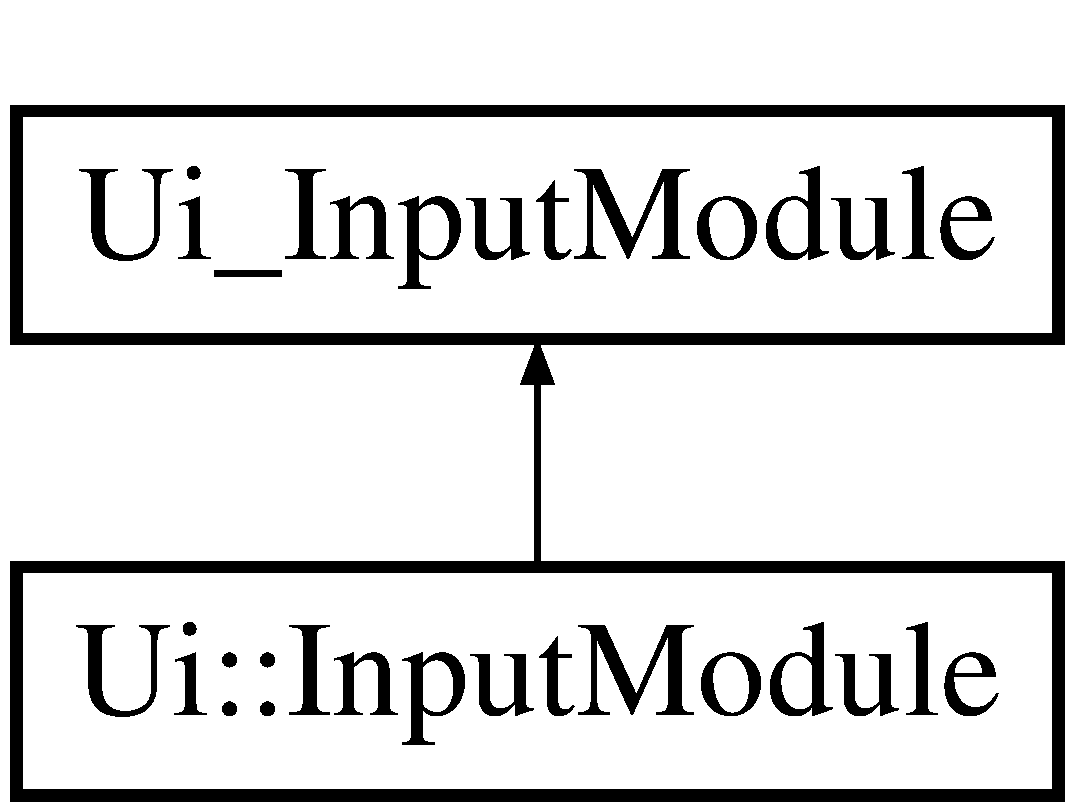
\includegraphics[height=2.000000cm]{class_ui___input_module}
\end{center}
\end{figure}
\subsection*{Public Member Functions}
\begin{DoxyCompactItemize}
\item 
\hypertarget{class_ui___input_module_aaf8f1500730e5aed8f431e0e2f369cab}{}void {\bfseries setup\+Ui} (Q\+Main\+Window $\ast$\hyperlink{class_input_module}{Input\+Module})\label{class_ui___input_module_aaf8f1500730e5aed8f431e0e2f369cab}

\item 
\hypertarget{class_ui___input_module_adea88dcba3a7d593bf259cf460cfd37c}{}void {\bfseries retranslate\+Ui} (Q\+Main\+Window $\ast$\hyperlink{class_input_module}{Input\+Module})\label{class_ui___input_module_adea88dcba3a7d593bf259cf460cfd37c}

\end{DoxyCompactItemize}
\subsection*{Public Attributes}
\begin{DoxyCompactItemize}
\item 
\hypertarget{class_ui___input_module_aff44a335ccc46a8bba6caaaf2407a954}{}Q\+Widget $\ast$ {\bfseries central\+Widget}\label{class_ui___input_module_aff44a335ccc46a8bba6caaaf2407a954}

\item 
\hypertarget{class_ui___input_module_a16d3b9a56396afd2d89b497b6fe7c583}{}Q\+Grid\+Layout $\ast$ {\bfseries grid\+Layout}\label{class_ui___input_module_a16d3b9a56396afd2d89b497b6fe7c583}

\item 
\hypertarget{class_ui___input_module_a42f60b85b6b9a3a7bffe5d63bffe776c}{}Q\+Spacer\+Item $\ast$ {\bfseries horizontal\+Spacer}\label{class_ui___input_module_a42f60b85b6b9a3a7bffe5d63bffe776c}

\item 
\hypertarget{class_ui___input_module_adb2c164f4259d5e09d919bf66fe85e9f}{}Q\+Label $\ast$ {\bfseries input\+Data\+Label}\label{class_ui___input_module_adb2c164f4259d5e09d919bf66fe85e9f}

\item 
\hypertarget{class_ui___input_module_a9ee3bc1119cc7022f034724d4c886b48}{}Q\+Spacer\+Item $\ast$ {\bfseries horizontal\+Spacer\+\_\+2}\label{class_ui___input_module_a9ee3bc1119cc7022f034724d4c886b48}

\item 
\hypertarget{class_ui___input_module_a9ee34cc594589b24e37ae831ae5ce8ff}{}Q\+Table\+Widget $\ast$ {\bfseries inv\+Proj\+Data\+Table\+Widget}\label{class_ui___input_module_a9ee34cc594589b24e37ae831ae5ce8ff}

\item 
\hypertarget{class_ui___input_module_a2673e00aa090f00149f9eeb8c326392c}{}Q\+Spacer\+Item $\ast$ {\bfseries horizontal\+Spacer\+\_\+5}\label{class_ui___input_module_a2673e00aa090f00149f9eeb8c326392c}

\item 
\hypertarget{class_ui___input_module_a0eec3d69a77652f71ca6251430544bc2}{}Q\+Push\+Button $\ast$ {\bfseries compare\+Invproj\+Push\+Button}\label{class_ui___input_module_a0eec3d69a77652f71ca6251430544bc2}

\item 
\hypertarget{class_ui___input_module_aafdff9d03c699a4c84a66bae9365c42c}{}Q\+Spacer\+Item $\ast$ {\bfseries horizontal\+Spacer\+\_\+7}\label{class_ui___input_module_aafdff9d03c699a4c84a66bae9365c42c}

\item 
\hypertarget{class_ui___input_module_a93740b54a6ed32b9a557270b49fc1079}{}Q\+Push\+Button $\ast$ {\bfseries make\+Inv\+Portfolio\+Push\+Button}\label{class_ui___input_module_a93740b54a6ed32b9a557270b49fc1079}

\item 
\hypertarget{class_ui___input_module_a5a72ab2ec61ba8000f838fa3ea5ba025}{}Q\+Menu\+Bar $\ast$ {\bfseries menu\+Bar}\label{class_ui___input_module_a5a72ab2ec61ba8000f838fa3ea5ba025}

\item 
\hypertarget{class_ui___input_module_abdf49f2ac11237a06a7df43b7b0d371a}{}Q\+Tool\+Bar $\ast$ {\bfseries main\+Tool\+Bar}\label{class_ui___input_module_abdf49f2ac11237a06a7df43b7b0d371a}

\item 
\hypertarget{class_ui___input_module_a2a340d851d9ea55f810e9244883ac6e2}{}Q\+Status\+Bar $\ast$ {\bfseries status\+Bar}\label{class_ui___input_module_a2a340d851d9ea55f810e9244883ac6e2}

\end{DoxyCompactItemize}


The documentation for this class was generated from the following file\+:\begin{DoxyCompactItemize}
\item 
C\+:/\+Users/\+Anton/\+Documents/\+Qt\+Projects/\+Investment\+Analysis\+Diploma/ui\+\_\+inputmodule.\+h\end{DoxyCompactItemize}

%--- End generated contents ---

% Index
\backmatter
\newpage
\phantomsection
\clearemptydoublepage
\addcontentsline{toc}{chapter}{Index}
\printindex

\end{document}
